\documentclass[thesis=B,czech,hidelinks]{thesis}[2012/06/26]

\usepackage[utf8]{inputenc}

\usepackage{algorithm2e}
\usepackage{amsthm}
\usepackage{dirtree}
\usepackage{fancyvrb}
\usepackage{graphicx}
\usepackage{listings}

\department{Katedra softwarového inženýrství}
\title{Implementace důkazového systému pro~výrokovou logiku}
\authorGN{Jan}
\authorFN{Švajcr}
\authorWithDegrees{Jan Švajcr}
\supervisor{Mgr. Jan Starý, Ph.D.}
\acknowledgements{Děkuji svému vedoucímu práce Mgr. Janu Starému, Ph.D. za přívětivost a~pomoc, své rodině za podporu a~zázemí a~své milované za lásku a~věrnost.}
\abstractCS{Cílem této práce je vypracovat terminálovou aplikaci implementující prostředí důkazového systému výrokové logiky. Její hlavní funkcionalitou je syntaktická analýza textového vstupu v~podobě posloupnosti výrokových formulí a~ověření, zdali je tato posloupnost korektním výrokovým důkazem. Software je implementován v~jazyce C++ a~je podporován prostředím UNIX. Součástí práce je dokumentace zdrojového kódu a~uživatelská příručka v~podobě standardní manuálové stránky.}
\abstractEN{The goal of this thesis is to create a~command line application implementing the proof system environment of the propositional logic. It's main functionality is parsing a~textual input representing a~sequence of propositional formulas and verifying this sequence as a~proof. The software is implemented in the C++ language and is supported by UNIX environment. Code documentation and a~standard manual page as a~user manual are also included.}
\placeForDeclarationOfAuthenticity{V~Praze}
\declarationOfAuthenticityOption{2}
\keywordsCS{Výroková logika, Důkazový systém, Parsing, C++.}
\keywordsEN{Propositional logic, Proof system, Parsing, C++.}

%
%
%

\begin{document}

\theoremstyle{definition}
\newtheorem{exm}{Příklad}
\newtheorem{dfn}{Definice}

\fvset{frame=single, numbers=left}

%
%
%

\begin{introduction}
Logika je formální věda zkoumající část lidského myšlení. Jejím předmětem je správné vyvozování důsledků z~předpokladů, jejichž volbu, pravdivost nebo snad smysl blíže nezkoumáme. Nečiníme tak nejen proto, že naše vyvození je správné i~v~případě, kdy předpoklady správné nejsou, ale i~proto, že to této disciplíně ani nepřísluší. Matematická logika toto usuzování formalizuje, čímž nás oprošťuje od psychologického aspektu. Dává tak vzniknout postupům, které lze kdykoliv opakovaně aplikovat. Příkladem takového postupu je ověřování správnosti našeho usuzování, tzv. důkazu. To je dokonce natolik mechanické, že jej můžeme svěřit strojovému zpracování\cite{sochor}. Právě tento aspekt výrokové logiky byl podnětem pro vznik této práce, která formalismus výrokové logiky implementuje počítačovým programem. Konkrétně implementuje principy Hilbertova systému. Ústřední kapitolou výrokového počtu, o~kterou se budeme v~rámci teoretické přípravy zajímat zejména, je \emph{dokazatelnost}.

Ještě předtím, než se ponoříme do problematiky implementace, je třeba analyzovat vlastnosti příslušné oblasti výrokového počtu. V~první kapitole proto vysvětlíme klíčové pojmy výrokové logiky, které nás budou provázet životním cyklem projektu a~budou tak pro nás nutnou znalostí. Pokračovat budeme kapitolou, ve které upřesníme zadání projektu a~vymezíme požadavky na implementaci. Následuje kapitola, ve které položíme základy pro vlastní implementaci. Budeme se zde věnovat rozkladu systému na menší celky a~návrhu jejich řešení. K~softwarové realizaci přejdeme v~navazující kapitole zabývající se technickými detaily samotné implementace. Nastíníme zde význam datových struktur a~popíšeme klíčové algoritmy. Předposlední kapitola se věnuje testování. Budeme se zde snažit maximálně pokrýt rizikové oblasti, které mohou ohrozit stabilitu aplikace. Práci zakončíme krátkým zamyšlením nad jejím možným pokračováním a~prodiskutujeme její rozšiřitelné stránky.
\end{introduction}

%
%
%

\chapter{Formální kontext}

V~úvodní kapitole se seznámíme s~několika základními pojmy výrokového počtu a~zavedeme terminologii užitou v~tomto textu, abychom na ni mohli čtenáře později odkázat. Tato část slouží jako teoretický základ celé práce. Čtenář znalý výrokové logiky ji může vynechat. Standardní terminologii, značení a~hlavní myšlenky přebíráme z~\cite{sochor} a~\cite{stary}.

\section{Výrok}

Nejprve zavedeme elementární pojem \emph{výrok}.

Výrok je takové tvrzení, o~kterém má smysl uvažovat, zdali je pravdivé, či nikoliv. Výrokům tedy přiřazujeme \emph{pravdivostní hodnoty} pravda (true) nebo nepravda (false).

\begin{exm}
Věta \uv{Dnes je hezký den.} je výrok. Je na čtenáři, aby rozhodl o~pravdivosti tohoto výroku. Jiný čtenář by mohl případně rozhodnout opačně.
\end{exm}
 
V~této práci se však pravdivostním ohodnocením výroků ani jejich významem nebudeme zabývat.

Výroková logika od vnitřní struktury výroků abstrahuje v~pojmu \emph{elementárního výroku}, ze kterých buduje \emph{výrokové formule} pomocí \emph{logických operací}. Jednotlivé elementární výroky značíme velkými písmeny latinky: $A, B, C, \ldots$

\section{Logické operace}

Logické operace dělíme na unární a~binární podle jejich arity\footnote{Arita -- počet operandů operace potřebných k~jejímu provedení.}. Symbolicky je reprezentují příslušné logické spojky následovně:

\begin{itemize}
	\item Unární
	\begin{description}
		\item[Negace] $\neg$
	\end{description}
	\item Binární
	\begin{description}
		\item[Konjunkce] $\wedge$
		\item[Disjunkce] $\vee$
		\item[Implikace] $\Rightarrow$
		\item[Ekvivalence] $\Leftrightarrow$
	\end{description}
\end{itemize}

Každá operace specificky určuje pravdivostní hodnotu složeného výroku v~závislosti na ohodnocení výroků, které pojí. Analogii s~logickými operátory lze vidět v~operátorech aritmetických. Význam uvedených operací nebudeme zkoumat, protože není pro účely této práce podstatný. Zkoumáme pouze výrokové formule a~jejich posloupnosti jako čistě syntaktické objekty.

\section{Formule}

Ústředním pojmem pro tuto práci je \emph{formule}.

\begin{dfn}
Ve výrokové logice definujeme formuli takto:
\begin{enumerate}
	\item Každá elementární formule je formulí.
	\item Vznikne-li $\alpha$ unární logickou operací z~formule $\beta$ nebo binární logickou operací z~formulí $\beta$ a~$\gamma$ , je $\alpha$ také formulí.
	\item Každá formule vznikne konečnou aplikací předchozích pravidel.
\end{enumerate}
\end{dfn}

Jednotlivé formule značíme malými písmeny řecké abecedy: $\alpha , \beta , \gamma , \ldots$

\begin{exm}
Pro ilustraci uvažujme dvě následující formule $\alpha, \beta$:
\begin{itemize}
	\item $\alpha = A$
	\item $\beta = \neg (A \vee B)$
\end{itemize}
Formule $\alpha$ je elementární formulí, kdežto formule $\beta$ je složená z~několika formulí. Pro názornost popíšeme výstavbu formule $\beta$ podle předchozí definice.
\begin{enumerate}
	\item $A$ a~$B$ jsou elementární formule (výroky).
	\item Formule $A, B$ pojí operace disjunkce do podoby složeného výroku $A \vee B$.
	\item Na dosavadní formuli aplikujeme unární operaci negace, čímž vznikne formule $\beta = \neg (A \vee B)$.
\end{enumerate}
\end{exm}

\subsection{Notace}

Nyní popíšeme několik způsobů zápisu výrokových formulí.

Výrokové formule lze zapisovat ve třech, sémanticky ekvivalentních, notacích: \emph{prefixní}, \emph{infixní} a~\emph{postfixní}. Tyto notace se liší pouze pořadím výpisu logické spojky ve složených výrocích.

\begin{exm}
Následující jsou různé zápisy téže formule:
\begin{description}
	\item[prefixní] $\neg \vee \alpha \: \beta$
	\item[infixní] $\neg (\alpha \vee \beta)$
	\item[postfixní] $\alpha \: \beta \vee \neg$
\end{description}
\end{exm}

Všimněme si, že v~případě prefixní a~postfixní notace je přednost operací určena jednoznačně na rozdíl od notace infixní, která vyžaduje užití závorek. Je třeba brát na vědomí, že s~rostoucí složitostí formule je pro nás čím dál obtížnější udržet pozornost nad její strukturou. Protože infixní zápis je našemu vnímání nejpřirozenější, budeme jej v~této práci používat i~nadále. Víme však, že kdykoliv lze jednu notaci převést na druhou.

\section{Důkazový systém}

\emph{Důkazový systém} výrokové logiky rozhoduje o~\emph{dokazatelnosti} výrokových formulí. Každý takový systém je tvořen dvěma součástmi:

\begin{itemize}
	\item Množinou axiomů
	\item Množinou odvozovacích pravidel
\end{itemize}

\emph{Axiomy} jsou schémata výrokových formulí jistého tvaru. Každou formuli ve tvaru popsaném axiomem nazýváme \emph{instancí} tohoto axiomu. Instancí axiomů je tedy nekonečně mnoho, stejně jako výrokových formulí.

Odvozovací pravidla popisují způsoby, jakými lze z~daných výrokových formulí odvozovat formule další.

\subsection{Hilbertův systém}
\label{sec:hilbert}

\emph{Hilbertův systém} je důkazový systém klasické výrokové logiky. Za účelem úspornosti jazyka se omezuje pouze na dvě logické spojky: negaci a~implikaci. Tyto dvě spojky tvoří tzv. \emph{minimální univerzální množinu}, proto všechny ostatní spojky můžeme vyjádřit těmito a~touto redukcí neomezujeme vyjadřovací možnosti jazyka. Způsob, jakým lze vyjadřovat jedny spojky pomocí druhých, zkoumat nebudeme.

Axiomem Hilbertova systému je každá formule některého z~následujících syntaktických tvarů:

\begin{description}
	\item[A1] $( \varphi \Rightarrow ( \psi \Rightarrow \varphi ))$
	\item[A2] $(( \varphi \Rightarrow ( \psi \Rightarrow \chi )) \Rightarrow (( \varphi \Rightarrow \psi ) \Rightarrow ( \varphi \Rightarrow \chi )))$
	\item[A3] $(( \neg \varphi \Rightarrow \neg \psi ) \Rightarrow (( \neg \varphi \Rightarrow \psi ) \Rightarrow \varphi ))$
\end{description}

Množina odvozovacích pravidel obsahuje jediný prvek, pravidlo \emph{modus ponens}, které je zavedeno následovně:

\begin{dfn}
Z~formulí $\varphi$ a~$\varphi \Rightarrow \psi$ odvoď formuli $\psi$.
\end{dfn}

V~této práci se nadále budeme zabývat výhradně tímto axiomatickým systémem. Existují však i~jiné důkazové systémy, které jsou navzájem ekvivalentní (viz část \ref{sec:gentzen}).

\subsection{Důkaz}

Nyní zavedeme klíčový pojem \emph{důkaz}.

\begin{dfn}
Buď $\varphi$ výroková formule. Řekneme, že konečná posloupnost výrokových formulí $\varphi_1 , \ldots, \varphi_n$ je \emph{důkazem} formule $\varphi$, pokud $\varphi_n$ je formule $\varphi$, a~každá formule $\varphi_i$ z~této posloupnosti je buďto instancí některého axiomu, nebo je z~některých předchozích $\varphi_j, \ldots , \varphi_k$, kde $j, \ldots , k < i$, odvozena odvozovacím pravidlem. Pokud existuje důkaz formule $\varphi$, řekneme, že je tato formule je \emph{dokazatelná} ve výrokové logice, a~píšeme $\vdash \varphi$.
\end{dfn}

Každý důkaz tedy nutně začíná axiomem a~triviálně každá instance axiomu je dokazatelnou formulí.

Pro nás klíčová je skutečnost, že důkaz vychází z~konečně mnoha daných předpokladů, postupuje dle konečně mnoha daných pravidel a~je v~každém kroku ověřitelný, což lze provést i~mechanicky. Na druhou stranu to nedává žádný návod, jak případně důkaz dané formule nalézt. Ostatně tato problematika již přesahuje rozsah této práce.

\begin{exm}
\label{exm:proof_a>a}
Pro ilustraci předvedeme důkaz formule $\varphi \Rightarrow \varphi$ v~Hilbertově systému.
\begin{description}
	\item[axiom 1] $(\varphi \Rightarrow ((\varphi \Rightarrow \varphi) \Rightarrow \varphi))$
	\item[axiom 2] $((\varphi \Rightarrow ((\varphi \Rightarrow \varphi) \Rightarrow \varphi)) \Rightarrow ((\varphi \Rightarrow (\varphi \Rightarrow \varphi)) \Rightarrow (\varphi \Rightarrow \varphi)))$
	\item[modus ponens, formule 1 a~2] $((\varphi \Rightarrow (\varphi \Rightarrow \varphi)) \Rightarrow (\varphi \Rightarrow \varphi))$
	\item[axiom 1] $(\varphi \Rightarrow (\varphi \Rightarrow \varphi))$
	\item[modus ponens, formule 4 a~3] $(\varphi \Rightarrow \varphi)$
\end{description}
\end{exm}

\subsubsection{Důkaz z~předpokladů}

Důkaz lze zobecnit na tzv. \emph{důkaz z~předpokladů} rozšířením stávající definice důkazu. Navíc zavedeme množinu \emph{předpokladů} $T$, tj. formulí, ze kterých v~rámci důkazu vycházíme. Zobecnění spočívá v~tom, že kromě axiomů jako členy důkazu obdobně připouštíme i~formule z~množiny předpokladů. Předpoklad je tedy formule, kterou, ačkoliv není axiomem, elementárně považujeme za dokazatelnou. Existuje-li důkaz formule $\varphi$ z~předpokladů $T$, píšeme $T \vdash \varphi$.

\subsubsection{Minimální důkaz}

Přirozený požadavek na jednoduchost vede k~otázce, zdali daný důkaz není v~nějakém smyslu zbytečně složitý. Například stočlenná posloupnost libovolných instancí axiomů je formálně korektním důkazem (svého posledního členu), který lze ovšem zkrátit na setinu původní délky. Podobně, pokud v~nějakém důkazu na náhodně zvoleném místě rozvineme nějaký jiný důkaz, vnikne posloupnost, která je opět formálně korektním důkazem, ovšem zbytečně složitým.

Ptáme se tedy, zdali předložený důkaz neobsahuje podobné \uv{zbytečnosti}, což nás vede k~pojmu \emph{minimální důkaz}.

\begin{dfn}
\label{dfn:minimal_proof}
Buď $\varphi_1, \ldots, \varphi_n$ posloupnost formulí tvořící důkaz formule $\varphi_n$. Tento důkaz nazveme \emph{minimálním}, pokud vynecháním libovolné formule posloupnosti $\varphi_1, \ldots, \varphi_n$ přestane důkaz být korektním.
\end{dfn}

Takový důkaz tedy neobsahuje zbytečné poddůkazy ani duplicitní formule, protože, pokud nějaká formule $\varphi_i$ vyplývá z~nějakých předchozích formulí pomocí odvozovacího pravidla, pak stejným způsobem vyplývá i~z~každých jejich předchozích, speciálně z~prvních, výskytů. Z~minimálního důkazu už nelze nic odstranit. To však neznamená, že neexistuje nějaký úplně jiný důkaz téže formule, který by byl ještě úspornější.

%
%
%

\chapter{Vymezení požadavků}

Na základě oficiálního zadání této práce, kterým začíná tento text, vymezíme v~této kapitole požadavky na implementovaný software. Tyto požadavky kategorizujeme na \emph{funkční} a~\emph{nefunkční}.

Funkční požadavky definují cíle, kterých má projekt dosáhnout. V~našem případě se jedná o~funkcionalitu námi implementovaného software. Na základě funkčních požadavků lze navrhnout metody testování a~ověřit úspěšné splnění zadání na konci projektu.

Mezi nefunkční požadavky řadíme náležitosti, které popisují způsob, jakým máme provést implementaci. Některé z~nich jsou součástí zadání, některé si pro úplnost zadání stanovíme sami. Nefunkční požadavky jsou omezení, ze kterých vycházíme, a~nejsou předmětem testování.

\section{Funkční požadavky}

Úkolem je vypracovat aplikaci \emph{pl} (propositional logic), která primárně dokáže rozhodnout, zdali je daná posloupnost výrokových formulí korektním formálním důkazem v~Hilbertově systému. Požadavkem nad rámec zadání je minimalizace těchto důkazů. Elementární funkcionalitou programu je syntaktická analýza vstupních formulí a~jejich případný výpis ve zvolené alternativní notaci a~jazyce. Nekorektní vstup program správně detekuje a~případně jeho nekorektnost podrobně hlásí.

Aplikaci je třeba náležitě otestovat a~metody užité při testování zdokumentovat. Dále je třeba vytvořit dokumentaci zdrojového kódu a~uživatelskou příručku k~aplikaci.

\section{Nefunkční požadavky}

\subsection{Aplikace}

Aplikace bude podporována na platformách systému UNIX a~implementována v~jazyce C++. Její obsluha bude možná přes systémový terminál, tedy nebude disponovat grafickým uživatelským rozhraním. To nepředstavuje žádné podstatné omezení funkcionality, neboť pracujeme pouze s~textovým vstupem. Veškerá funkcionalita aplikace bude dostupná standardně pomocí přepínačů příkazové řádky. Vstupní data budou aplikaci předávána buďto na standardním vstupu, anebo v~textovém souboru. Návratová hodnota programu bude signalizovat úspěšnost výsledku.

\subsection{Vstup}

Aplikace čte buďto ze standardního vstupu nebo ze souboru textový ASCII vstup v~podobě posloupnosti řádek obsahujících výrokové formule zapsané ve stanoveném jazyce. Podporován je prefixní, infixní i~postfixní zápis formulí. Vstup nevyhovující stanovené formě je považován za nekorektní a~je odmítnut.

\subsection{Výstup}

Forma výstupu závisí na zvolené funkcionalitě, ke které je program nakonfigurován při spuštění. Podporován je výpis formulí v~prefixní, infixní i~postfixní notaci. Výstupní jazyk formulí může mít podobu ASCII znaků, přirozeného jazyka nebo jazyka \LaTeX{}. Výstupem programu může být v~určitých případech chybové hlášení o~nekorektním vstupu.

\subsection{Dokumentace}

Programátorská dokumentace bude dostupná v~podobě HTML stránek za použití nástroje \emph{Doxygen}, který takovou dokumentaci generuje. Zdrojový kód programu proto opatříme komentáři speciálního stylu, který tento nástroj vyžaduje.

\subsection{Příručka}

Uživatelskou příručku realizujeme v~podobě standardní manuálové stránky operačních systémů UNIX. Tato stránka bude po instalaci přístupná standardně pomocí příkazu \texttt{man pl}.

%
%
%

\chapter{Analýza a~návrh}

\section{Technický kontext}

V~této části popíšeme technologie, které jsme pro implementaci stanovili nefunkčními požadavky, a~odůvodníme jejich užití.

\subsection{C++}

Programovací jazyk C++ je rozšířením jazyka C. Vybrali jsme jej zejména proto, že podporuje objektově-orientované paradigma, kterého se budeme držet. Přednosti tohoto programovacího stylu nám usnadní nejen implementaci, ale i~návrh.

Pro jazyk C++ existuje velké množství standardních knihoven, které nabízejí běžné funkce či běžné datové typy. Jejich užití vede k~úspoře zdrojového kódu a~menší míře zanesených chyb. Při implementaci budeme maximálně využívat těchto standardních knihoven. Zejména využijeme knihovny STL obsahující šablony základních kontejnerů. Naopak, nebudeme využívat prostředky třetích stran.

Při implementaci také dbáme na přenositelnost a~rozšiřitelnost aplikace, jak požaduje zadání.

\subsubsection{C++11}

C++11 je jedním z~posledních standardů jazyka C++. Vybrali jsme jej především z~důvodu úspory kódu, což umožňují některé konstrukty, které tento standard zavedl, zejména např. alternativní zápis cyklu \texttt{for}, který abstrahuje od iterátorů při procházení kontejnerů\cite{cpp}.

\subsection{Make}

Nástroj \texttt{make} slouží k~zjednodušení sestavování programů. Jeho předností je zejména schopnost na základě časové známky určit, které součásti programu je třeba zkompilovat v~případě změny zdrojového kódu. Sestavení tento nástroj řídí konfiguračním souborem \texttt{Makefile}. Ten má předepsanou strukturu a~obsahuje definice pravidel, tzv. \emph{cílů}, které mají svůj název a~konkrétní účel. Cíl je definován posloupností příkazů pro \texttt{shell}, které jsou provedeny při jeho volání. Každý cíl může navíc obsahovat \emph{závislosti}. Závislost je další cíl, který je volán přednostně. Speciálními (konečnými) cíli bývá kompilace konkrétního zdrojového souboru.

My použijeme nástroj GNU \texttt{make}, který je jednou z~implementací klasického \texttt{make} rozšířenou o~pokročilé funkce. Z~nich konkrétně využijeme např. \emph{pattern rules}, \emph{wildcard characters} či \emph{string functions}\cite{gmake}.

\subsection{Doxygen}

Doxygen je nástroj pro automatickou tvorbu dokumentace zdrojového kódu. Umožňuje dokumentovat kód mnohých populárních programovacích jazyků, zejména C++. Podporuje různé formy výstupu, přičemž my zvolíme dokumentaci v~podobě HTML stránek. Text dokumentace tento nástroj čerpá přímo ze souborů zdrojového kódu prostřednictvím speciálních komentářů. To zajišťuje neustálou konzistenci mezi dokumentací a~zdrojovým kódem. Tento nástroj funguje i~v~případě nezdokumentovaného kódu, kdy alespoň podá základní přehled o~prvcích zdrojového kódu. V~neposlední řadě je schopen vizualizovat relace mezi elementy v~podobě diagramů, jako je např. diagram tříd\cite{doxygen}.

My budeme dokumentaci zapisovat především do hlavičkových souborů \texttt{.hpp}, aby nepřekážela v~implementaci.

\subsection{Mdoc}

Manuálové stránky systému UNIX lze psát ve speciálním značkovacím jazyce. Takový jazyk je ve skutečnosti balíček maker pro jazyk \emph{troff}. Troff pochází ze 70. let a~podobně jako např. \TeX{} slouží k~sazbě textu. Jazyk zpracovává stejnojmenný textový procesor, který podporuje právě zmíněné balíčky maker pro tento jazyk. Jednotlivá makra, podobně jako např. značky jazyka HTML, formátují daný obsah do požadované podoby\cite{troff}. Běžné manuálové stránky užívají balíček maker \texttt{man}. My však zvolíme sofistikovanější balíček \texttt{mdoc}, který narozdíl od \texttt{man} disponuje sémantickou koncepcí maker. Záznam o~tomto balíčku nalezneme v~sekci \emph{mdoc(7)} manuálových stránek\cite{mdoc}.

Aby manuálová stránka byla dostupná pomocí příkazu \texttt{man}, musí splňovat určité náležitosti. Název souboru manuálové stránky má následující formát:

\begin{center}
\texttt{[název aplikace].[manuálová sekce]}
\end{center}

Stejnojmenný archiv souboru s~manuálovou stránkou je umístěn v~adresáři, ve kterém příkaz \texttt{man} implicitně hledá manuálové stránky\footnote{Tato umístění zobrazíme, popř. nastavíme pomocí příkazu \texttt{manpath}.} pod adresářem příslušícím dané manuálové sekci. V~našem případě se jedná o~adresář \texttt{man1}. Absolutní cesta k~naší manuálové stránce může vypadat například následovně: \texttt{/usr/local/man/man1/pl.1.gz}. Soubor archivu s~manuálovou stránkou má vlastníka uživatele \texttt{root} a~přístupová práva 0644.

Manuálové stránky mají standardní strukturu, kterou dodržíme. Text příručky napíšeme v~angličtině a~její obsah rozdělíme do příslušných standardních sekcí.

\section{Případy užití}

Na základě funkčních požadavků nastíníme možné případy užití aplikace (viz obrázek \ref{fig:use_cases}).

\begin{figure}
\centering
\caption{Diagram případů užití}
\label{fig:use_cases}
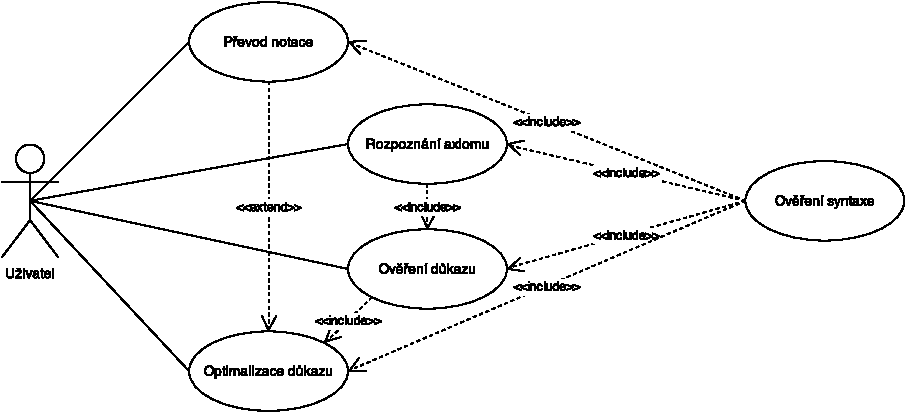
\includegraphics[width=\linewidth]{diagrams/use_cases}
\end{figure}

\subsection{Převod notace}

Elementární funkcionalitou aplikace je převod formulí dané notace do notace vybrané. Zároveň je tato funkcionalita vhodná i~pro kontrolu syntaktického zápisu formulí. Forma logických spojek výstupu je dostupná v~podobě znaků ASCII (stejně jako vstup), v~přirozeném jazyce nebo v~jazyce \LaTeX{}.

\subsection{Rozpoznání axiomu}

Protože součástí ověření důkazu je rozpoznání axiomů, nabídneme tuto funkci také samostatně. Každá formule vstupní posloupnosti je potom ověřována jako axiom a~na výstupu je případně uváděn jeho typ.

\subsection{Ověření důkazu}

Tato funkcionalita je hlavním cílem této práce. Na vstupní posloupnost formulí je nahlíženo jako na posloupnost členů důkazu, přičemž aplikace ověří, zdali je důkaz korektním. Je možné ověřovat i~důkaz z~předpokladů. Tehdy je prvních $n$ vstupních formulí považováno za prvky teorie, pak následují formule vlastního důkazu. Výstupem aplikace jsou podrobnosti o~dokazatelnosti, popř. nedokazatelnosti každého členu důkazu.

\subsection{Minimalizace důkazu}

Důkaz je nejprve ověřen stejně jako v~předchozím případě. Následně, pokud je to možné, je minimalizován do nejúspornější možné podoby (viz definici \ref{dfn:minimal_proof}). Výstupem je důkaz téže formule právě v~této podobě.

\section{Návrh}

\subsection{Forma vstupu}

Textový vstup aplikace \texttt{pl} se skládá z~posloupnosti formulí, přičemž každá z~nich je zakončena řádkovým zalomením \texttt{\textbackslash n}. Zápis formulí užívá znaků \texttt{A-Z} pro elementární výroky. Tím je vstup omezen na 26 různých elementárních výroků, což ovšem pro naše účely plně postačuje. Symboly \texttt{-}, \texttt{.}, \texttt{+}, \texttt{>}, \texttt{=} značí po řadě logické operátory negace, konjunkce, disjunkce, implikace a~ekvivalence. Pro infixní notaci formulí navíc rozpoznáváme závorky \texttt{()} pro určování přednosti operací.

\subsection{Forma výstupu}

Kromě výstupní notace lze zvolit i~jednu ze tří výstupních forem (jazyků) logických spojek. Jak jsou jednotlivé operátory zastoupeny v~těchto jazycích, znázorňuje tabulka \ref{tab:connectives_language}.

\begin{table}
\centering
\caption{Výstupní formy logických spojek}
\label{tab:connectives_language}
\begin{tabular}{|c||c|c|c|}\hline
Operátor & ASCII & Slovní & \LaTeX{} \tabularnewline \hline \hline
Negace & \verb|-| & \verb|not| & \verb|\neg| \tabularnewline \hline
Konjunkce & \verb|.| & \verb|and| & \verb|\wedge| \tabularnewline \hline
Disjunkce & \verb|+| & \verb|or| & \verb|\vee| \tabularnewline \hline
Implikace & \verb|>| & \verb|implies| & \verb|\Rightarrow| \tabularnewline \hline
Ekvivalence & \verb|=| & \verb|iff| & \verb|\Leftrightarrow| \tabularnewline \hline
\end{tabular}
\end{table}

\subsection{Uživatelské rozhraní}

Nefunkčním požadavkem na uživatelské rozhraní je obsluha pomocí přepínačů. V~této části tedy navrhneme přepínače aplikace \texttt{pl} pokrývající veškerou funkcionalitu stanovenou v~požadavcích. 

\begin{description}
	\item[-A] (axiom checker) Ověří vstupní formule jako axiomy.
	\item[-e] (echo) Povolí hlášení na standardním a~standardním chybovém výstupu. Implicitně není produkován žádný výstup.
	\item[-f file] (input file) Použije soubor \emph{file} jako vstup namísto (implicitního) standardního vstupu.
	\item[-i syntax] (input syntax) Nastaví danou vstupní notaci formulí. Možné hodnoty jsou: \emph{prefix}, \emph{infix} a~\emph{postfix}. Implicitní hodnota je \emph{infix}.
	\item[-l language] (output language of connectives) Nastaví danou výstupní formu jazyka logických spojek. Možné hodnoty jsou: \emph{ascii}, \emph{words} a~\emph{latex}. Implicitní hodnota je \emph{ascii}.
	\item[-o syntax] (output syntax) Nastaví danou výstupní notaci formulí. Možné hodnoty jsou: \emph{prefix}, \emph{infix} a~\emph{postfix}. Implicitní hodnota je \emph{infix}.
	\item[-M n] (proof minimizer) Minimalizuje důkaz ze vstupní posloupnosti formulí. Parametr \emph{n} vyjadřuje počet formulí množiny předpokladů, které na vstupu předcházejí samotnému důkazu.
	\item[-P n] (proof checker) Ověří důkaz ze vstupní posloupnosti formulí. Parametr \emph{n} vyjadřuje počet formulí množiny předpokladů, které na vstupu předcházejí samotnému důkazu.
	\item[-s] (strict) Způsobí zastavení vykonávání programu při prvním neúspěchu, např. nekorektním syntaktickém zápisu formule. Přepínače \texttt{-M} a~\texttt{-P} takové chování povolují automaticky, protože nemá smysl dále minimalizovat či ověřovat evidentně nekorektní důkaz.
\end{description}

\emph{Axiom checker}, \emph{proof checker} a~\emph{proof minimizer} budeme nazývat \emph{cíli} aplikace. Volba cíle je nepovinná, je však povoleno spustit aplikaci s~jediným zvoleným cílem.

%
%
%

\chapter{Implementace}

V~této kapitole popíšeme, jak ty které části zdrojového kódu implementují jednotlivé součásti systému. Zmíníme však pouze ty nejdůležitější z~nich.

\section{Hlavní program}

Hlavní program aplikace představuje funkce \texttt{main}.

\paragraph{main}

Inicializací instance třídy \texttt{Configuration} dojde ke konfiguraci aplikace dle parametrů příkazové řádky. V~případě úspěchu je proveden cíl aplikace. V~případě, že se nepodaří aplikaci nakonfigurovat, je vypsáno chybové hlášení a~běh aplikace končí neúspěchem.

\section{Popis tříd}

V~této části vysvětlíme význam jednotlivých funkcí, tříd a~jejich metod. Následující text koresponduje s~dokumentací zdrojového kódu.

\subsection{Třída Configuration}

Tato třída představuje konfiguraci aplikace. Obsahuje proměnné, které řídí její běh.

\paragraph{Konstruktor}

Pomocí funkce \texttt{getopt} z~knihovny \texttt{unistd.h} jsou zpracovány přepínače z~příkazové řádky, podle kterých jsou nastaveny třídní proměnné.

\paragraph{parseFormula}

Tato metoda zavolá příslušný parser formulí, kterému předá příslušný vstupní proud.

\paragraph{printFormula}

Tato metoda vrátí textovou podobu dané formule v~příslušné notaci a~jazyce logických spojek.

\subsection{Třída ExecutionTarget}

Tato abstraktní třída představuje cíl aplikace. Hierarchii tříd rodiny \texttt{ExecutionTarget} znázorňuje diagram \ref{fig:execution_target}.

\begin{figure}
\centering
\caption{Diagram tříd rodiny ExecutionTarget}
\label{fig:execution_target}
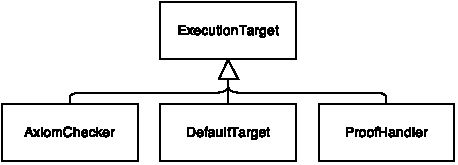
\includegraphics{diagrams/execution_target}
\end{figure}

\paragraph{executeTarget}

Účelem této abstraktní metody je provést cíl v~závislosti na konfiguraci aplikace a~vrátit příslušnou návratovou hodnotu. Základem všech implementací této metody je cyklické zpracování formulí vstupní posloupnosti, které vždy začíná přijetím formule metodou \texttt{parseFormula}. V~případě nekorektního vstupu je mimo cyklus zachycena výjimka typu \texttt{ParseException} a~vypsáno chybové hlášení získané metodou \texttt{getMessage}. Některé cíle v~rámci cyklu zohledňují konfigurační příznak \texttt{strict} a~v~případě neúspěšné iterace cyklus předčasně zastavují.

\subsubsection{AxiomChecker}

Tato třída představuje cíl axiom checker.

\paragraph{executeTarget}

Přijatá vstupní formule je v~rámci daného důkazového systému metodou \texttt{isAxiom} ověřena jako axiom. Následuje uvolnění formule z~paměti a~výpis hlášení o~shodě či neshodě s~konkrétním typem axiomu.

\subsubsection{DefaultTarget}

Tato třída představuje stav spuštění bez explicitního cíle.

\paragraph{executeTarget}

Přijatá vstupní formule je vypsána na výstupu pomocí metody \texttt{printFormula} a~následně je uvolněna z~paměti.

\subsubsection{ProofHandler}

Tato třída představuje cíle proof checker a~proof minimizer.

\paragraph{executeTarget}

Určitý počet přijatých vstupních formulí je nejprve zařazen mezi prvky teorie. Tyto formule totiž ještě nejsou členy vlastního důkazu. Zbylé formule jsou zpracovány následovně.

Přijatá formule je postupně ověřena jako axiom metodou \texttt{isAxiom}, jako prvek teorie a~jako formule odvoditelná v~rámci daného důkazového systému metodou \texttt{isDeducible}. Každá formule splňující jedno z~těchto kritérií je přidána do seznamu prvků třídy \texttt{ProofMember} představujícího důkaz. Nesplňuje-li formule ani jedno z~uvedených kritérií, důkaz není korektním a~aplikace končí neúspěchem. Je-li instance \texttt{ProofHandler} nastavena jako cíl proof minimizer, následuje iterativní algoritmus minimalizace důkazu.

Inicializujeme zásobník prvků třídy \texttt{ProofMember} a~uložíme na něj poslední člen důkazu. Dokud není zásobník prázdný, prohlašujeme jeho vrchol členem minimálního důkazu metodou \texttt{setPreserve} a~jeho přímé svědky ukládáme na zásobník. Zároveň sledujeme počet takto zpracovaných prvků. Je-li na konci tento počet shodný s~počtem členů důkazu, důkaz již byl minimálním, tedy nelze jej minimalizovat.

\begin{algorithm}
\KwData{$Z$ je zásobník členů důkazu}
ulož poslední člen důkazu na $Z$\;
\While{$Z$ není prázdný}
{
	vrchol $Z$ je členem minimálního důkazu\;
	\ForEach{svědek $s$ vrcholu $Z$}
	{
		ulož $s$ na $Z$\;
	}
}
\end{algorithm}

Členy důkazu, které jsme označili jako členy minimálního důkazu, vypíšeme na výstup.

\subsection{Třída Formula}

Struktura výrokové formule má stromový charakter, a~proto jsme ji implementovali jako \emph{syntaktický strom}. Tato abstraktní třída představuje uzel tohoto stromu, tedy dílčí formuli celého výrazu. Objekt této třídy obsahuje znak reprezentující uzel jako logickou spojku nebo výrok. Hierarchii tříd rodiny \texttt{Formula} znázorňuje diagram \ref{fig:formula}.

\begin{figure}
\centering
\caption{Diagram tříd rodiny Formula}
\label{fig:formula}
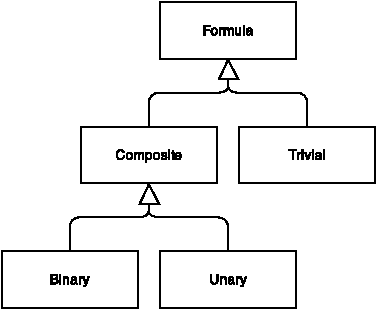
\includegraphics{diagrams/formula}
\end{figure}

\paragraph{equals}

Účelem této abstraktní metody je zjistit, zdali se daná formule shoduje s~touto.

\paragraph{matches}

Účelem této abstraktní metody je zjistit, zdali daná formule vyhovuje tvaru určenému touto formulí.

\subsubsection{Třída Composite}

Tato abstraktní třída představuje formuli složenou z~logické spojky a~příslušných operandů. Znak reprezentující tento uzel stromu je jednou z~logických spojek.

\subsubsection{Třída Trivial}

Tato třída představuje triviální formuli, tedy elementární výrok. Znak reprezentující tento uzel stromu je jedním ze symbolů pro výroky.

\paragraph{equals}

Implementace spočívá v~porovnání reprezentujícího znaku této a~dané formule.

\paragraph{matches}

Implementace spočívá v~porovnání metodou \texttt{equals} dané formule s~formulí, která je substitucí za reprezentující znak této formule. Tyto substituce se vyhledávají v~mapě substitucí, jejíž reference je předána parametrem metody \texttt{matches}. Pokud se v~této mapě doposud nenachází substituce za reprezentující symbol této formule, do mapy je tento symbol vložen jako klíč a~daná formule jako jeho hodnota a~metoda vrátí \texttt{true}.

\begin{algorithm}
\KwData{$s$ je reprezentující symbol této formule, $\varphi$ je daná formule, $T$ je tabulka substitucí}
\If{v~$T$ se nachází klíč $s$}
{
	\KwRet{formule $T(s)$ se shoduje s~formulí $\varphi$}\;
}
\Else
{
	do $T$ dosaď dvojici $\{s, \varphi\}$\;
	\KwRet{true}\;
}
\end{algorithm}

\subsubsection{Třída Binary}

Tato třída představuje binární operátor. Objekt této třídy obsahuje odkaz na svůj levý a~pravý operand, tedy levého a~pravého potomka tohoto uzlu v~syntaktickém stromu formule.

\paragraph{equals}

Implementace spočívá v~porovnání reprezentujícího symbolu této a~dané formule a~následném porovnání shody levého a~pravého operandu této formule metodou \texttt{equals} s~levým a~pravým operandem formule dané.

\begin{algorithm}
\KwData{$\varphi$ je daná formule}
\If{reprezentující symboly této formule a~$\varphi$ se shodují}
{
	přetypuj $\varphi$ na objekt typu \texttt{Binary}\;
	\KwRet{levý operand této formule se shoduje s~levým operandem formule $\varphi$ a~zároveň pravý operand této formule se shoduje s~pravým operandem formule $\varphi$}\;
}
\end{algorithm}

\paragraph{matches}

Implementace spočívá v~porovnání reprezentujícího symbolu této a~dané formule a~následném porovnání tvaru levého a~pravého operandu této formule metodou \texttt{matches} s~levým a~pravým operandem formule dané.

\begin{algorithm}
\KwData{$\varphi$ je daná formule}
\If{reprezentující symboly této formule a~$\varphi$ se shodují}
{
	přetypuj $\varphi$ na objekt typu \texttt{Binary}\;
	\KwRet{levý operand této formule vyhovuje tvaru levého operandu $\varphi$ a~zároveň pravý operand této formule vyhovuje tvaru pravého operandu $\varphi$}\;
}
\end{algorithm}

\subsubsection{Třída Unary}

Tato třída představuje formuli složenou unárním operátorem. Objekt této třídy obsahuje odkaz na svůj operand, tedy potomka tohoto uzlu v~syntaktickém stromu formule.

\paragraph{equals}

Implementace spočívá v~porovnání reprezentujícího symbolu této a~dané formule a~následném porovnání shody operandu této formule metodou \texttt{equals} s~operandem formule dané.

\paragraph{matches}

Implementace spočívá v~porovnání reprezentujícího symbolu této a~dané formule a~následném porovnání tvaru operandu této formule metodou \texttt{matches} s~operandem formule dané.

\subsection{Parser formulí}

Parserem abstraktně nazveme tu část programu, která převádí vstup z~textové do vnitřní formy. V~našem případě jej reprezentují samostatné funkce \emph{parsePrefix}, \emph{parseInfix} a~\emph{parsePostfix}. Každá z~těchto funkcí slouží ke zpracování vstupních formulí v~příslušné notaci. V~případě úspěchu funkce vrací kořen syntaktického stromu přijaté formule.

Syntaktická analýza postupuje v~cyklu po jednotlivých znacích vstupního proudu, aby mohla být přerušena již v~místě případné syntaktické chyby, tedy ještě před přijetím celého vstupu. Nyní popíšeme algoritmy syntaktické analýzy korektního vstupu těchto funkcí.

\paragraph{parsePrefix}

Prefixní parser ukládá přijaté logické operátory na zvláštní zásobník s~operátory. Po přijetí elementární formule je tato nastavena jako operand zleva vrcholu zásobníku. Ve chvíli, kdy jsou operandy vrcholu zásobníku již plně obsazeny, dojde k~sejmutí operátoru ze zásobníku. Tento operátor je pak nastaven jako operand zleva novému vrcholu zásobníku. To se opakuje, dokud aktuální vrchol zásobníku opět nedisponuje alespoň jedním volným operandem.

\paragraph{parseInfix}

Infixní parser ukládá přijaté logické operátory na zvláštní zásobník s~operátory a~elementární formule na zvláštní zásobník s~formulemi. K~orientaci ve struktuře formule využívá další zásobník se stavy zpracování větví syntaktického stromu. Každá taková úroveň zpracování může mít následující stav:

\begin{description}
	\item[UNARY] Byl nastaven unární operátor. 
	\item[BLANK] Byla otevřena nová větev stromu.
	\item[FIRST\_OPERAND] Byl nastaven první operand.
	\item[BINARY] Byl nastaven binární operátor.
	\item[LAST\_OPERAND] Byl nastaven poslední operand.
\end{description}

Podle těchto stavů lze na základě jistých pravidel vždy rozhodně určit, zdali aktuálně zpracovávaný prvek neporušuje infixní syntaxi formulí. Taková pravidla popisují chování infixního parseru v~závislosti na přijatém prvku a~stavu zpracování aktuální větve stromu.

\paragraph{parsePostfix}

Postfixní parser ukládá přijaté elementární formule na zvláštní zásobník s~formulemi. Ve chvíli, kdy je přijat logický operátor, dojde k~sejmutí příslušného počtu formulí ze zásobníku, přičemž tyto jsou zprava nastaveny jako operandy přijatého operátoru. Ten je následně uložen na zásobník.

\subsection{Třída ParseException}

Tato obecná třída představuje výjimku při syntaktické analýze v~případě nekorektního vstupu. Objekt této třídy obsahuje řetězec s~popisem syntaktické chyby. Hierarchii výjimek rodiny \texttt{ParseException} znázorňuje diagram \ref{fig:parse_exception}.

\begin{figure}
\centering
\caption{Diagram tříd rodiny ParseException}
\label{fig:parse_exception}
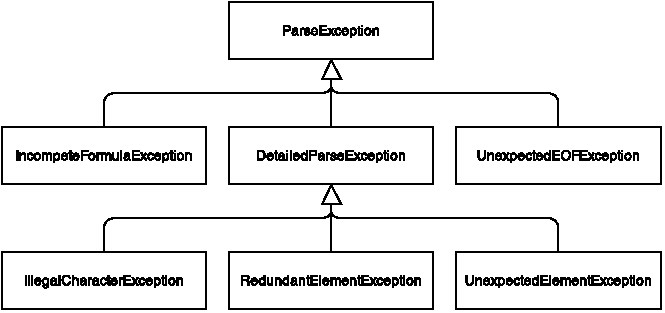
\includegraphics[width=\linewidth]{diagrams/parse_exception}
\end{figure}

\paragraph{getMessage}

Tato metoda vrátí podrobnosti o~chybě v~podobě řetězce s~chybovým hlášením.

\subsubsection{Výjimka DetailedParseException}

Tento obecný typ výjimky představuje syntaktickou chybu specifikovanou znakem vstupu, který chybu způsobil, a~jeho pozici na řádce (nepočítaje bílé znaky).

\subsubsection{Výjimka IncompleteFormulaException}

Tento typ výjimky představuje případ nekompletní formule.

\subsubsection{Výjimka UnexpectedEOFException}

Tento typ výjimky představuje případ výskytu konce vstupu v~místě, které není stanoveno korektní formou vstupu.

\subsubsection{Výjimka IllegalCharacterException}

Tento typ výjimky představuje případ užití nepovoleného znaku.

\subsubsection{Výjimka RedundantElementException}

Tento typ výjimky představuje případ výskytu nadbytečných prvků nacházejících se za korektní formulí.

\subsubsection{Výjimka UnexpectedElementException}

Tento typ výjimky představuje případ nekorektního zápisu formule (týká se pouze infixní notace).

\subsection{Třída ProofMember}

Tato třída představuje člen důkazu jako komplexní strukturu. Objekt této třídy obsahuje výrokovou formuli jakožto člen důkazu, seznam přímých svědků tohoto členu a~logickou proměnnou \texttt{preserve} vyhrazenou pro algoritmus minimalizace důkazu.

\subsection{Třída ProofSystem}

Tato abstraktní třída představuje důkazový systém výrokové logiky. Objekt této třídy obsahuje axiomy důkazového systému. Hierarchii tříd rodiny \texttt{ProofSystem} znázorňuje diagram \ref{fig:proof_system}.

\begin{figure}
\centering
\caption{Diagram tříd rodiny ProofSystem}
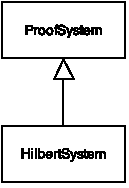
\includegraphics{diagrams/proof_system}
\label{fig:proof_system}
\end{figure}

\paragraph{isAxiom}

Účelem této metody je ověřit, zdali je daná formule instancí některého z~axiomů důkazového systému. Implementace spočívá v~porovnání dané formule s~jednotlivými typy axiomů pomocí metody \texttt{matches}.

\begin{algorithm}
\KwData{$\psi$ je daná formule}
\ForEach{axiom $\alpha$ důkazového systému}
{
	\If{$\psi$ vyhovuje tvaru $\alpha$}
	{
		\KwRet{typ axiomu $\alpha$}\;
	}
}
\KwRet{false}\;
\end{algorithm}

\paragraph{isDeducible}

Účelem této abstraktní metody je ověřit, zdali je daná formule dokazatelná z~předchozích kroků daného důkazu. Metoda je abstraktní, protože každý konkrétní důkazový systém odvozuje formule jiným způsobem, resp. odvozovacím pravidlem. Návratovou hodnotou je posloupnost indexů členů důkazu, ze kterých je daná formule odvoditelná. Tato posloupnost je prázdná v~případě, že formuli v~rámci daného důkazu odvodit nelze.

\subsubsection{Třída HilbertSystem}

Tato třída představuje Hilbertův systém. Pro účely odvozování formulí obsahuje objekt této třídy formuli představující implikaci pravidla modus ponens ($\varphi \Rightarrow \psi$).

\paragraph{isDeducible}

Implementace spočívá v~procházení jednotlivých formulí daného důkazu, přičemž na jednu z~formulí je nahlíženo jako na předpoklad pravidla modus ponens ($\varphi$) a~na druhou jako na jeho implikaci ($\varphi \Rightarrow \psi$). Daná formule ($\psi$) je odvoditelná, je-li nalezena dvojice formulí vyhovující právě těmto tvarům.

\begin{algorithm}
\KwData{$\psi$ je daná formule}
\ForEach{formule $\alpha$ důkazu}
{
	\ForEach{formule $\beta$ důkazu}
	{
			\If{$\beta$ vyhovuje tvaru $\alpha \Rightarrow \psi$}
			{
				\KwRet{indexy formulí $\alpha$, $\beta$}\;
			}
	}
}
\end{algorithm}

\subsection{Třída UsageException}

Tato obecná třída představuje výjimku při konfiguraci aplikace v~případě nesprávné syntaxe příkazové řádky. Objekt této třídy obsahuje záznam o~tom, který přepínač syntaktickou chybu způsobil, a~řetězec s~popisem této chyby. Hierarchii výjimek rodiny \texttt{UsageException} znázorňuje diagram \ref{fig:usage_exception}.

\begin{figure}
\centering
\caption{Diagram tříd rodiny UsageException}
\label{fig:usage_exception}
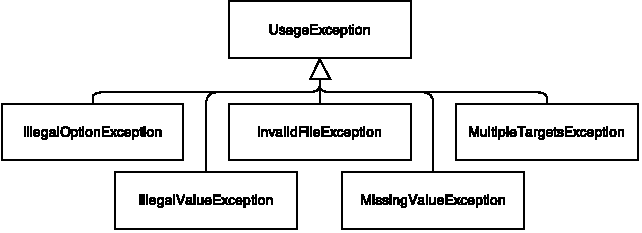
\includegraphics{diagrams/usage_exception}
\end{figure}

\paragraph{getMessage}

Tato metoda vrátí podrobnosti o~syntaktické chybě v~podobě řetězce s~chybovým hlášením.

\subsubsection{Výjimka IllegalOptionException}

Tento typ výjimky představuje případ použití nepovoleného přepínače.

\subsubsection{Výjimka IllegalValueException}

Tento typ výjimky představuje případ použití nepovolené hodnoty přepínače.

\subsubsection{Výjimka InvalidFileException}

Tento typ výjimky představuje případ zadání nepoužitelného vstupního souboru.

\subsubsection{Výjimka MissingValueException}

Tento typ výjimky představuje případ vynechání povinné hodnoty přepínače.

\subsubsection{Výjimka MultipleTargetsException}

Tento typ výjimky představuje případ zadání více cílů k~provedení najednou.

%
%
%

\chapter{Testování}

V~této kapitole popíšeme užité metody testování aplikace, jak požaduje zadání. Testovali jsme oblasti pokryté případy užití:

\begin{itemize}
	\item Zpracování vstupu.
	\begin{itemize}
		\item Ověření syntaxe.
		\item Převod notace.
	\end{itemize}
	\item Rozpoznání axiomu.
	\item Ověření důkazu.
	\item Minimalizaci důkazu.
\end{itemize}

Základní myšlenkou pro maximalizaci pokrytí případů testy je v~každé této oblasti provést následující typy testů:

\begin{description}
	\item[Pozitivní test] Test korektního přijetí korektního vstupu.
	\item[Negativní test] Test korektního odmítnutí nekorektního vstupu.
\end{description}

Princip všech testů spočívá ve zpracování připravených vstupních dat a~následné konfrontaci výstupu aplikace s~připravenými výstupními testovacími daty, která považujeme za korektní. Touto konfrontací myslíme porovnání těchto dat pomocí nástroje \texttt{diff}. Vstupní a~výstupní testovací data jsme uložili do textových souborů do adresáře \texttt{test}.

Vlastní testy jsou technicky realizovány skriptem pro \texttt{shell}. Spuštění tohoto testovacího skriptu volá cíl \texttt{make test}. Soubory s~příponou \texttt{\_test} vyprodukované testy jsou směrovány do adresáře \texttt{out}.

\section{Zpracování vstupu}

Všechny případy užití aplikace zahrnují užití parseru výrokových formulí. Proto jsme nejdříve ze všeho ověřili, zdali parser korektně transformuje korektní textový vstup do stanovené vnitřní reprezentace a~nekorektní vstup korektně odmítá. To jsme zjistili porovnáním vstupních dat s~výstupními daty téže notace. Protože parser v~naší implementaci reprezentují tři nezávislé funkce (\texttt{parsePrefix}, \texttt{parseInfix} a~\texttt{parsePostfix}), bylo nezbytné testovat vstupní data všech tří notací. 

\subsection{Pozitivní test}

Pozitivní test ověřuje korektní převod formulí každé ze tří notací vstupu do každé ze tří notací výstupu.

\subsubsection{Vstupní data}

Připravili jsme dostatečný počet různých výrokových formulí tak, abychom jimi pokryli následující případy:

\begin{itemize}
	\item Kořenem stromu je:
	\begin{itemize}
		\item Elementární formule
		\item Složená formule
		\begin{itemize}
			\item Unární operátor
			\item Binární operátor
		\end{itemize}
	\end{itemize}
	\item Potomek uzlu je:
	\begin{itemize}
		\item Elementární formule
		\item Složená formule
		\begin{itemize}
			\item Unární operátor
			\item Binární operátor
		\end{itemize}
	\end{itemize}
\end{itemize}

Vstupními testovacími daty (pro infixní notaci) je následující posloupnost formulí:

\VerbatimInput{../impl/test/parser_infix_pos_in.txt}

\subsubsection{Výstupní data}

Výstupními testovacími daty (pro infixní notaci) jsou tatáž data.

\subsection{Negativní test}

Negativní test ověřuje korektní odmítnutí nekorektního vstupu. Nekorektní vstup však může mít mnoho podob, jež bylo třeba analyzovat. K~tomu nám posloužil výčet druhů výjimek rodiny \texttt{ParseException} vrhaných parserem.

\subsubsection{Vstupní data}

Připravili jsme dostatečný počet různých nekorektních výrokových formulí tak, abychom jimi pokryli následující případy:

\begin{enumerate}
	\item Formule je nekompletní.
	\item Formule má chybnou syntaxi (pouze infixní notace).
	\item Formule obsahuje nadbytečné prvky.
	\item Formule obsahuje nepovolený znak.
	\item Formule není korektně ukončena.
\end{enumerate}

Vstupními testovacími daty (pro infixní notaci) je následující posloupnost formulí:

\VerbatimInput{../impl/test/parser_infix_neg_in.txt}

\subsubsection{Výstupní data}

Výstupními testovacími daty (pro infixní notaci) je následující posloupnost hlášení:

\VerbatimInput{../impl/test/parser_infix_neg_out.txt}

\section{Rozpoznání axiomu}

Pro testování rozpoznání axiomů jsme využili axiomy Hilbertova systému.

\subsection{Pozitivní test}

Pozitivní test ověřuje korektní rozpoznání axiomů všech typů.

\subsubsection{Vstupní data}

Vstupními testovacími daty je následující posloupnost formulí:

\VerbatimInput{../impl/test/axiom_checker_pos_in.txt}

\subsubsection{Výstupní data}

Výstupními testovacími daty je následující posloupnost hlášení:

\VerbatimInput{../impl/test/axiom_checker_pos_out.txt}

\subsection{Negativní test}

Negativní test ověřuje korektní odmítnutí formulí zdánlivě podobných axiomům.

\subsubsection{Vstupní data}

Vstupními testovacími daty je následující posloupnost formulí:

\VerbatimInput{../impl/test/axiom_checker_neg_in.txt}

\subsubsection{Výstupní data}

Výstupními testovacími daty je následující posloupnost chybových hlášení:

\VerbatimInput{../impl/test/axiom_checker_neg_out.txt}

\section{Ověření důkazu}

Pro testování ověření důkazu jsme využili pozměněný důkaz formule $A \Rightarrow A$ z~příkladu \ref{exm:proof_a>a}.

\subsection{Pozitivní test}

Pozitivní test ověřuje korektní ověření značně neminimálního avšak korektního důkazu.

\subsubsection{Vstupní data}

Vstupními testovacími daty je následující posloupnost formulí:

\VerbatimInput{../impl/test/proof_checker_pos_in.txt}

\subsubsection{Výstupní data}

Výstupními testovacími daty je následující posloupnost hlášení:

\VerbatimInput{../impl/test/proof_checker_pos_out.txt}

\subsection{Negativní test}

Negativní test ověřuje korektní odmítnutí nekorektního důkazu.

\subsubsection{Vstupní data}

Vstupními testovacími daty je následující posloupnost formulí:

\VerbatimInput{../impl/test/proof_checker_neg_in.txt}

\subsubsection{Výstupní data}

Výstupními testovacími daty je následující posloupnost hlášení:

\VerbatimInput{../impl/test/proof_checker_neg_out.txt}

\section{Minimalizace důkazu}

Pro testování ověření důkazu jsme využili pozměněný důkaz formule $A \Rightarrow A$ z~příkladu \ref{exm:proof_a>a}.

\subsection{Pozitivní test}

Pozitivní test ověřuje korektní minimalizaci značně neminimálního důkazu.

\subsubsection{Vstupní data}

Vstupními testovacími daty je následující posloupnost formulí:

\VerbatimInput{../impl/test/proof_checker_pos_in.txt}

\subsubsection{Výstupní data}

Výstupními testovacími daty je následující posloupnost formulí:

\VerbatimInput{../impl/test/proof_minimizer_pos_out.txt}

\subsection{Negativní test}

Negativní test ověřuje korektní odmítnutí již minimálního důkazu.

\subsubsection{Vstupní data}

Vstupními testovacími je následující posloupnost formulí:

\VerbatimInput{../impl/test/proof_minimizer_pos_out.txt}

\subsubsection{Výstupní data}

Výstupními testovacími daty je následující hlášení:

\VerbatimInput{../impl/test/proof_minimizer_neg_out.txt}

\section{Další testy}

Kromě testů korektní funkčnosti aplikace jsme ověřili následující náležitosti.

\subsection{Test uvolnění paměti}

Programy psané v~jazyce C++ vyžadují explicitní správu paměti již ve zdrojovém kódu. Pro detekci paměťových úniků za běhu aplikace a~ověření uvolnění veškeré alokované paměti na konci jejího běhu jsme použili nástroj \texttt{valgrind}. Aplikaci jsme ručně spouštěli s~testovacími daty a~zjištěné nedostatky odstranili.

\subsection{Test manuálové stránky}

Jazyk manuálových stránek má stanovenou formu. Korektní manuálová stránka proto musí dodržovat správnou syntaxi maker a~např. také nesmí obsahovat prázdné řádky. K~ověření korektnosti manuálové stránky jsme použili procesor GNU \texttt{troff}:

\begin{lstlisting}
groff -z -mdoc
\end{lstlisting}

\subsection{Test přenositelnosti}

Aplikaci jsme úspěšně otestovali na následujících operačních systémech:

\begin{itemize}
	\item Debian 7.5 (i386)
	\item FreeBSD 10.0 (amd64)
	\item OpenBSD 5.5 (i386, amd64, macppc)
	\item OpenBSD 5.4 (amd64)
	\item MacOSX 10.5.8 (intel)
	\item Ubuntu 14.04 (amd64)
\end{itemize}

Jelikož při implementaci používáme konstrukty jazyka C++ ve standardu C++11, potřebujeme k~sestavení aplikace překladač, který je zdrojový kód v~této podobě schopen přeložit. Takový překladač však neexistuje na některých dalších systémech, což do jisté míry omezuje další (pohodlnou) přenositelnost.

%
%
%

\chapter{Rozšiřitelnost}

Po implementaci dosavadní funkcionality se nabízí některá přirozená rozšíření, která však přesahují zadání práce i~časové možnosti. V~této kapitole některá z~těchto rozšíření uvedeme a~nastíníme jejich možné začlenění do obsluhy aplikace.

\section{Nalezení důkazu}

Tato práce nás naučila \emph{ověřovat} důkazy výrokových formulí v~Hilbertově systému. Nezabývali jsme se však otázkou, jakým způsobem důkazy \emph{hledat}. Naši implementaci by velice obohatila právě funkcionalita nalezení důkazu dané (dokazatelné) formule.

Pro nalezení důkazu bychom využili rozhodnutelnosti logiky, tedy skutečnosti, že dokazatelné jsou právě tautologie\footnote{Tautologie -- výroková formule, která je vždy pravdivá.}, a~ty se dají efektivně poznat. Je totiž zřejmé, že hledat důkaz formule má smysl až tehdy, když zjistíme, že je dokazatelná.

Vztah mezi výpočetní složitostí procedury, která výrokové důkazy \emph{ověřuje} (takovou proceduru jsme implementovali), a~složitostí procedury, která výrokové důkazy \emph{nachází}, je hlubokou otevřenou otázkou teoretické informatiky. Je totiž jednou z~populárních reformulací tzv. \emph{PNP problému}. Tyto souvislosti jdou ovšem značně nad rámec našeho zadání, a~proto jsme se jimi nezabývali. Namísto toho odkazujeme čtenáře na \cite{krajicek} a~\cite{cook}.

\subsection{Návrh obsluhy}

Zavedeme nový přepínač \texttt{-F} (find a~proof).

Přepínač \texttt{-F} je novým cílem aplikace \texttt{pl}. Při jeho použití jsou vstupní formule vnímány jako formule, ke kterým chceme nalézt důkaz. Aplikace se jej pokusí nalézt a~případně jej vypíše na výstup.

\section{Gentzenův systém}
\label{sec:gentzen}

V~části \ref{sec:hilbert} jsme zmínili, že Hilbertův systém není jediným formálním důkazovým systémem výrokové logiky. Pravidlo modus ponens však zřejmě nejlépe odpovídá postupům našeho uvažování\cite{sochor}. Existují ovšem i~jiná formální odvozovací pravidla, např. \emph{pravidlo rezoluce}, které zavádí \emph{Gentzenův systém}.

Stávající implementaci bychom mohli rozšířit právě o~tento důkazový systém. Aplikace by tak mohla důkazy v~tomto systému ověřovat, minimalizovat nebo je mezi těmito systémy převádět.

\subsection{Pravidlo rezoluce}

Pravidlo rezoluce používá jazyk logických spojek odlišný od jazyka Hilbertova systému. Je zavedeno následovně\cite{stary}:

\begin{dfn}
Z~formulí $\varphi \vee \alpha$ a~$\neg \psi \vee \vartheta$ odvoď formuli $\psi \vee \vartheta$.
\end{dfn}

Každou takto odvozenou formuli nazýváme \emph{rezolventou}.

\subsection{Návrh obsluhy}

\subsubsection{Režim důkazového systému}

Zavedeme nový přepínač \texttt{-r} (deduction rule).

Přepínač \texttt{-r} s~hodnotami \texttt{hilbert} a~\texttt{gentzen} je rozšířením stávající funkcionality práce s~důkazy. Určuje, kterému důkazovému systému náleží vstupní důkaz, který chceme ověřit nebo minimalizovat.

\subsubsection{Překlad důkazů}

Zavedeme nový přepínač \texttt{-C} (convert).

Přepínač \texttt{-C} s~hodnotami \texttt{hilbert} a~\texttt{gentzen} je novým cílem aplikace. Při jeho použití aplikace přeloží vstupní důkaz do podoby daného výstupního důkazového systému. Protože systémy Hilbertův a~Gentzenův jsou ekvivalentní\cite{stary} a~překlad důkazů v~těchto systémech je rutinní\cite{sochor}, úspěch překladu závisí pouze na korektnosti vstupního důkazu.

\section{Paralelní práce}

Zadání této bakalářské práce vychází z~velkého množství požadavků na tutéž aplikaci \texttt{pl}. Z~těchto požadavků byly sestaveny tři zadání bakalářských prací, které byly vypracovávány paralelně. Funkcionalita ostatních částí se měla týkat také např. sémantiky výrokové logiky, kterou jsme se v~této práci nezabývali. Jaké možné pokračování této práce, stejně jako těch dvou dalších, se proto nabízí sjednocení funkcionality těchto tří aplikaci do jediné, což je původní motivace.

%
%
%

\begin{conclusion}
Tato práce mi dala možnost uplatnit mnohé znalosti, které mi předala Fakulta informačních technologií ČVUT v~Praze během mého bakalářského studia. Zejména jsem uplatnil programovací dovednost v~jazyce C++, dokumentaci kódu ve stylu Doxygen, sestavování programu pomocí nástroje \texttt{make}, sazbu textu v~\LaTeX{} a~znalost v~oblasti výrokové logiky. Své dosavadní znalosti jsem navíc rozšířil. Nových znalostí jsem nabyl konkrétně v~oblasti tvorby manuálových stránek pro systém UNIX pomocí balíčku maker \texttt{mdoc}. V~neposlední řadě jsem si poprvé zkusil literární činnost v~tomto rozsahu.
\end{conclusion}

%
%
%

\bibliographystyle{csn690}
\bibliography{bibliography}

\appendix

%
%
%

\chapter{Seznam použitých zkratek}

\begin{description}
	\item[ASCII] American Standard Code for Information Interchange
	\item[GNU] GNU's Not Unix
	\item[HTML] HyperText Markup Language
	\item[STL] Standard Template Libraries
\end{description}

%
%
%

\chapter{Obsah přiloženého CD}

\begin{figure}
\dirtree{%
	.1 src\DTcomment{adresář se zdrojovou formou práce}.
	.2 impl\DTcomment{adresář se zdrojovou formou implementace}.
	.3 doc\DTcomment{adresář se soubory HTML dokumentace}.
	.3 src\DTcomment{adresář se soubory zdrojového kódu}.
	.3 test\DTcomment{adresář se soubory pro testování}.
	.3 Doxyfile\DTcomment{soubor konfigurace nástroje Doxygen}.
	.3 Makefile\DTcomment{soubor konfigurace nástroje make}.
	.3 pl.1\DTcomment{soubor zdrojové formy manuálové stránky}.
	.3 test.sh\DTcomment{soubor testovacího skriptu pro shell}.
	.2 thesis\DTcomment{adresář se zdrojovou formou textu práce}.
	.1 text\DTcomment{adresář s~texty práce}.
}
\end{figure}

\chapter{Instalační příručka}

Adresář \texttt{src/impl} uložte na svůj disk a~přejděte do pracovního adresáře \texttt{impl}. Následuje popis cílů nástroje GNU \texttt{make}, které nyní lze spouštět.

\begin{description}
	\item[build] Sestaví aplikaci. Binární formu aplikace \texttt{pl} naleznete po spuštění tohoto cíle v~adresáři \texttt{out}. K~úspěšnému sestavení je nutné, aby váš \texttt{gcc} kompilátor podporoval standard C++11.
	\item[clean] Odstraní veškeré výstupy vyprodukovaných při práci s~\texttt{make}. Spuštění tohoto cíle vrátí adresář \texttt{impl} do původního stavu.
	\item[doc] Vygeneruje programátorskou dokumentaci ve formátu HTML. Dokumentaci naleznete po spuštění tohoto cíle v~adresáři \texttt{doc}. Tento cíl vyžaduje přítomnost nástroje \texttt{doxygen} v~systému.
	\item[install] Sestaví a~nainstaluje do systému aplikaci a~manuálovou stránku. K~úpravě instalačního umístění změňte proměnnou \texttt{PREFIX} v~souboru \texttt{Makefile} na požadovanou hodnotu. Pokud instalujeme do systémového umístění, je k~instalaci nutné mít oprávnění uživatele \texttt{root}. Po instalaci je aplikace dostupná odkudkoliv pomocí příkazu \texttt{pl} a~manuálová stránka pomocí příkazu \texttt{man pl}.
	\item[test] Sestaví a~otestuje aplikaci za využití testovacích souborů v~adresáři \texttt{test}. Testování končí hlášením o~úspěšnosti testů. Soubory vyprodukované testy naleznete po spuštění tohoto cíle v~adresáři \texttt{out}.
	\item[uninstall] Odinstaluje aplikaci a~manuálovou stránku ze systému, pokud do něj předtím byla nainstalována spuštěním cíle \texttt{install}. 
\end{description}

\end{document}
